\documentclass{article}
\usepackage[utf8]{inputenc}
\usepackage[absolute,overlay]{textpos}
\usepackage{graphicx}
\usepackage{caption}
\usepackage{subfig}
\usepackage[a4paper, margin={1.91cm, 2.54cm}]{geometry}

\begin{document}


\begin{textblock*}{6cm}(14.6cm,1cm) % {block width} (coords) 
    \begin{flushright}
    \normalsize Cafer SELLİ 2444974\\\normalsize Zeynep Beril ŞAHİN 2587848    
    \end{flushright}
\end{textblock*}

\begin{center}
\huge IE206-Term Project I\\\Large Spring 2022
\end{center}


\tableofcontents


\addcontentsline{toc}{section}{Introduction}
\section*{Introduction}

\; \; Due to the pandemic, humanity learned that it was not even prepared for any kind of disasters nature could release upon us. Predicting and simulating an upcoming disaster could be a significant game-changer for the favor of humankind. Especially disasters such as pandemics and epidemics look like a completely random system at first glance, but in a virtual environment, their behavior can be observed with high precision.

This project is a pandemic simulation for a grid-based environment. By moving the main elements, people in the population, with a random-walk principle based on uniform distribution, our simulation embraces the everyday movements of the people that can not be predicted. Also, by adjusting different parameters that could be a solution to the epidemic, such as vaccination or isolation, predicting the behavior of the virus could be possible.

Predicting the behavior of the virus enables decision-makers to develop and implement more efficient pandemic policies, which may be crucial for the well-being of the population during the pandemic. The aim of this project is to create environments for implementing different policies and comparing them in terms of results on the population.

\addcontentsline{toc}{section}{PART I : Interpretation of Graphs}
\section*{PART I : Interpretation of Graphs}

\; \; \;In Scenario I (Figure \ref{fig:totalAll}.a), almost all of the population (240 people) got infected by the virus. Even if there are quarantine restrictions, the spread of the virus is still not under control. In less than 30 iterations, all of the population is infected by the virus. So quarantine restrictions by themselves are not enough for such a case. On the other hand, however, in Scenario II (Figure \ref{fig:totalAll}.b), some of the population is not even infected by the virus. At the end of 120 iterations, approximately 30 people out off 240 (Obtained by running the Monte-Carlo simulation 100 times) are not even getting infected by the virus. 

Compared with Scenario I, the effect of vaccination is more significant than the quarantine. Even if the movement of an infected person could be restricted, there is still a probability of them roaming around and infecting others. With these two graph, in order to reduce the \textbf{total} number of infected people, we can use a vaccination policy rather than an isolation policy.

However, by examining the per iteration data of Scenario I and II, the difference between each policy can be seen clearly. For the Scenarios I and II, in the Figure \ref{fig:perIter1&2}, there is a single spike that emerges at iteration 15 on the Scenario I with a peak of 15 people per iteration, but in Scenario II, there are two different spikes with a peak of each is greater than 40 person per iteration. 

These spikes can also be observed in the death rates per iteration. The total number of deceased people in Scenario I and Scenario II is similar to each other, but in Scenario I, this number mostly emerged in a single wave. However, in Scenario II, it is spread across two waves. The number of healed people per iteration follows a similar sequence in both scenarios.


\begin{figure}[h]
    \centering
    \subfloat[\centering Scenario I]{{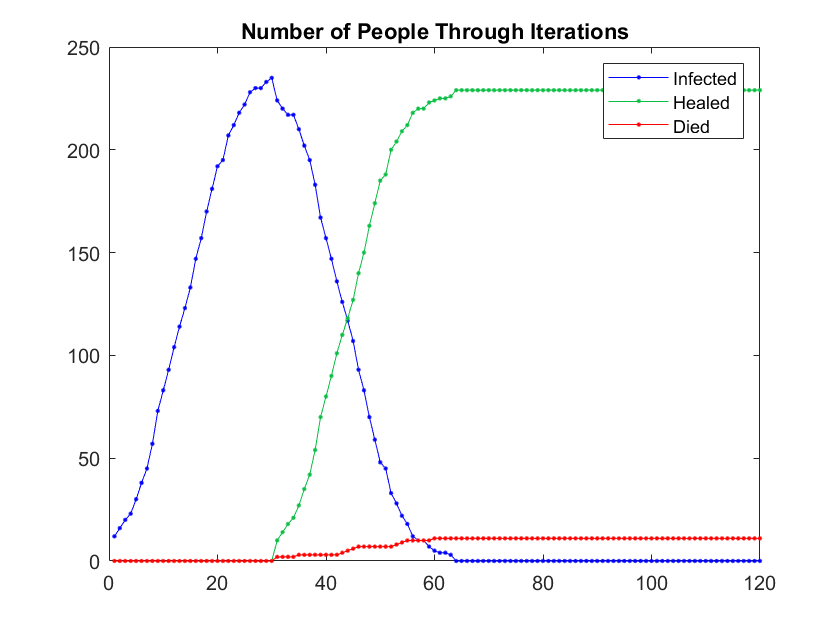
\includegraphics[width=6cm]{images/ScenarioI_overall.png} }}%
    \qquad
    \subfloat[\centering Scenario II]{{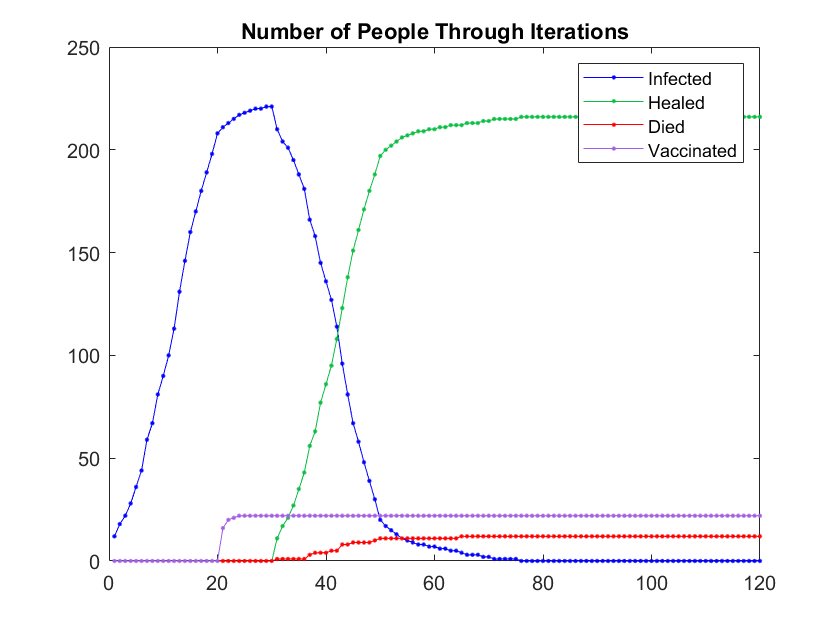
\includegraphics[width=6cm]{images/ScenarioII_overall.png} }}%
    \qquad
    \subfloat[\centering Scenario III]{{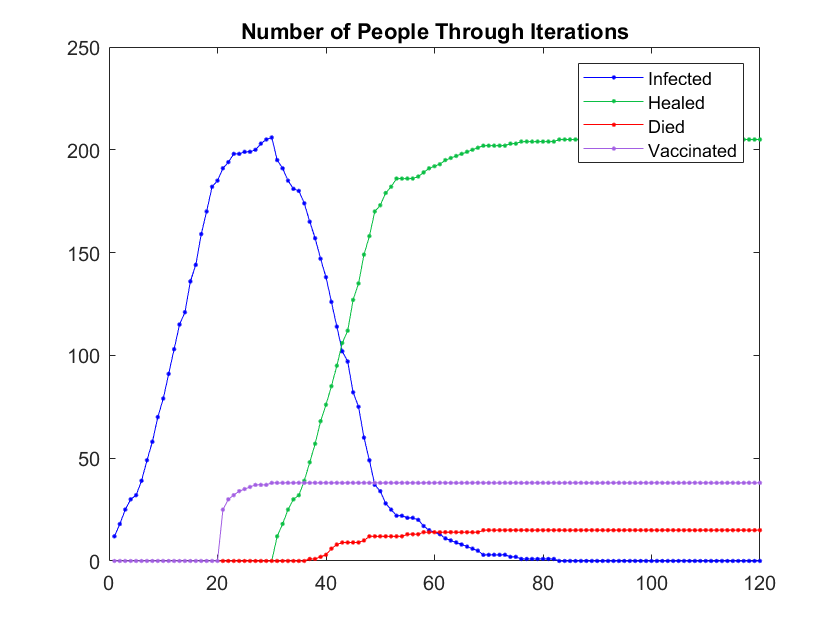
\includegraphics[width=6cm]{images/ScenarioIII_overall.png} }}%
    \qquad
    \subfloat[\centering Scenario IV]{{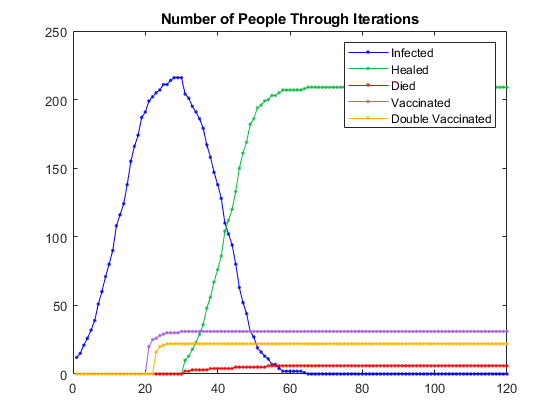
\includegraphics[width=6cm]{images/ScenarioIV_overall.png} }}%
    \caption{Total number of each people trough iterations}%
    \label{fig:totalAll}%
\end{figure}

In Scenario I, the pandemic is spread across a wider iteration period and reaches an end in a single wave. With such a wide-ranged event, the failure of the healthcare system might be averted, but the drawback of this Scenario is all of the population is still getting infected. This situation is prevented in Scenario II with vaccination. However, due to the huge spikes, healthcare systems might fail due to this high increase in the number of infected people per iteration.

\begin{figure}[h]
    \centering
    \subfloat[\centering Scenario I]{{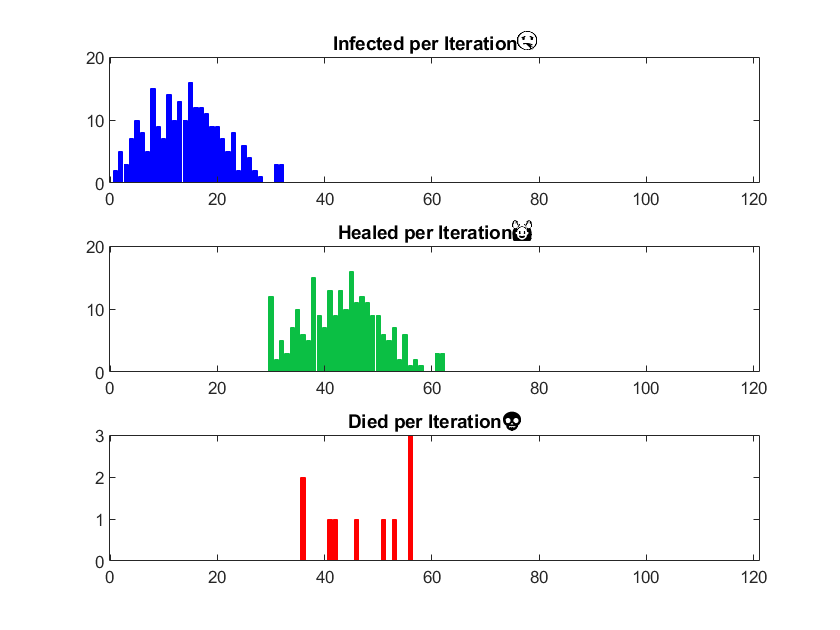
\includegraphics[width=8cm]{images/ScenarioI_PerIteration.png} }}%
    \qquad
    \subfloat[\centering Scenario II]{{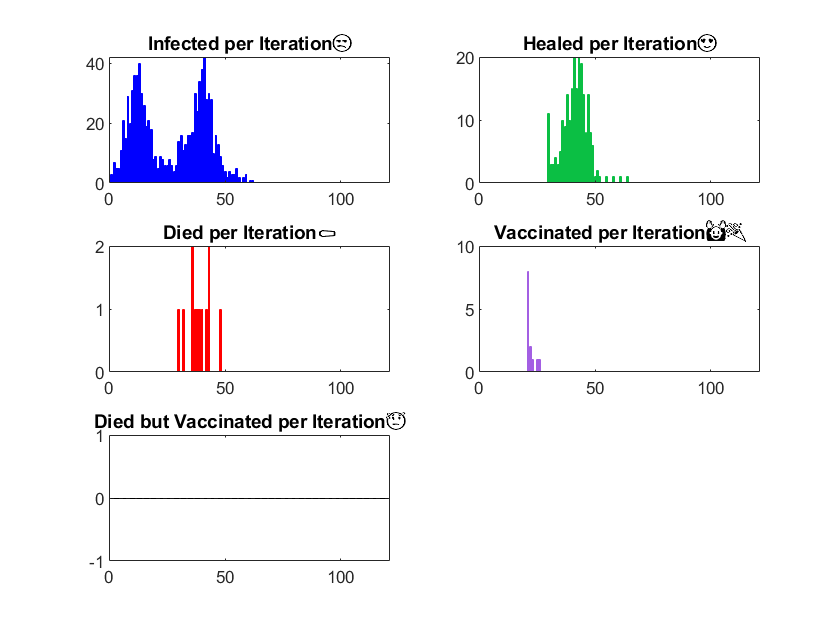
\includegraphics[width=8cm]{images/ScenarioII_PerIteration.png} }}%
    \caption{Number of people in each iteration for Scenario I \& II}
    \label{fig:perIter1&2}%
\end{figure}

Scenario III solves both of the problems in Scenario I and Scenario II by combining aspects of both. Using both vaccination and quarantine policy, the peak point of the total number of infected people, in Figure \ref{fig:totalAll}.c, lowered almost to 200 people. That means approximately 17\% of the population is not even infected by the virus. Also, in Figure \ref{fig:perIter3&4}.a, the peak of infected per iteration is decreased to 15 people per iteration. This is a huge relief for the healthcare system in our simulation.

\newpage

\begin{figure}[h]
    \centering
    \subfloat[\centering Scenario III]{{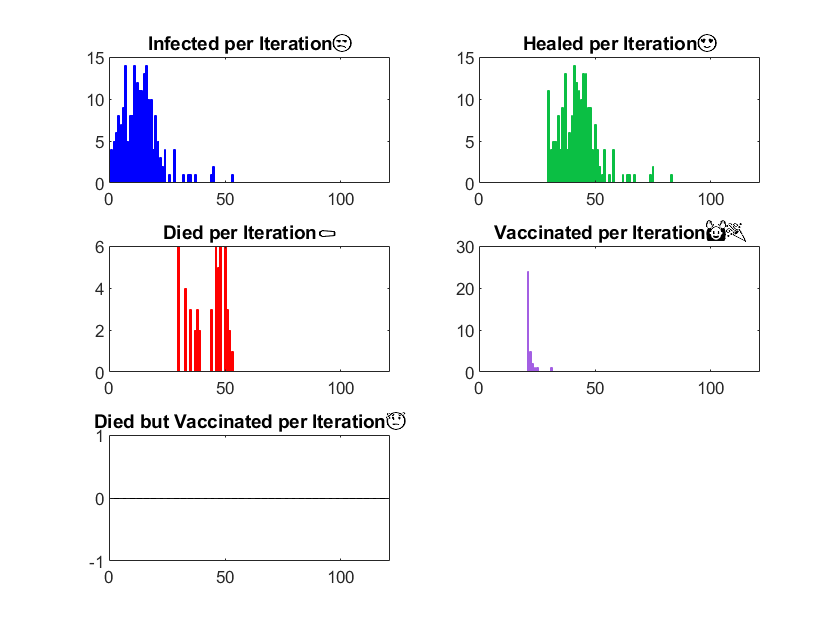
\includegraphics[width=8cm]{images/ScenarioIII_PerIteration.png} }}%
    \qquad
    \subfloat[\centering Scenario IV]{{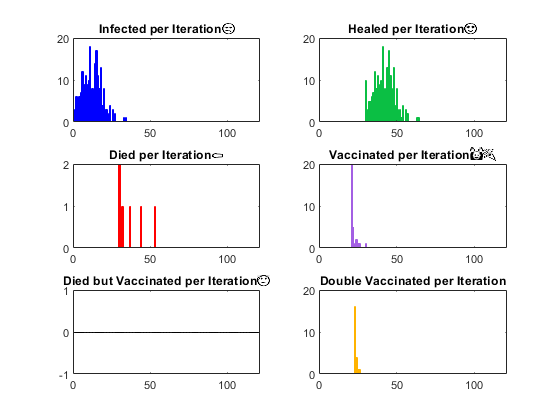
\includegraphics[width=8cm]{images/ScenarioIV_PerIteration.png} }}%
    \caption{Number of people in each iteration for Scenario III \& IV}
    \label{fig:perIter3&4}%
\end{figure}

Since both quarantine and vaccination are used, the number of total vaccinated people is increased by approximately 10 people. A similar relation holds for the vaccinated per iteration too. The number of people who died but were vaccinated per iteration almost sits at the 0 level because someone with vaccination has only a 5\% chance of getting the virus. In addition to that, it is 5\%, so the overall chance of vaccinated people dying from the virus is 0.25\%. This is why those who died but were vaccinated per iteration level stayed at 0.

Scenario IV adds another dimension to the simulation with the double vaccination policy. With a double vaccination policy, each individual has an 80\% probability of having the second dose of vaccination. Assuming that if they are not vaccinated for the second time after exactly 3 iterations, their protection against the virus wares out (i.e., their probability of getting infected will be equal to 50\% rather than 5\%). Also, they will not be eligible for the second dose. Due to this, the total number of infected people in the population is still equal to the value of Scenario III. 

However, due to the wear out of vaccination, some people get infected after they are vaccinated, and this leads to infection of more people overall. Peak values of the infected number of people per iteration are lower than Scenario III, but this difference can only be observed on average.

The biggest impact of the double vaccination policy is decreasing the total death rate of the pandemic. Since any double vaccinated person is completely immune to the virus, this leads to decreasing the death chance of an individual to 0 without any consequences. In Figure \ref{fig:totalAll}.d dramatic drop in the total death is clearly seen. The same effect is also visible in the death per iteration rate. In Figure \ref{fig:perIter3&4}.b, died per iteration rate is less frequent and has smaller peak values due to the double vaccination.

Another impact of double vaccination is decreasing the infected but vaccinated amount. This result actually has two causes. The first one is that the people that do not want to take the second dose are excluded from the vaccinated list. The second reason is that individuals that took the second dose are completely immune to the virus.
\newpage
\addcontentsline{toc}{section}{PART II : Alternative Scenarios}
\section*{PART II : Alternative Scenarios}

\addcontentsline{toc}{subsection}{Isolation Probability ( Scenario I )}
\subsection*{Isolation Probability ( Scenario I )}

\; \; Under only the isolation policy implemented, the effect of isolation probability is examined by changing the original isolation probability. By setting the value to higher and lower values, the total number of infected and dead people through the iterations is graphed according to the simulation (Figure \ref{fig:AlterQSSC1})
\begin{figure}[h]
    \centering
    \subfloat[\centering Isolation Probability ($q_s$) = 0.2]{{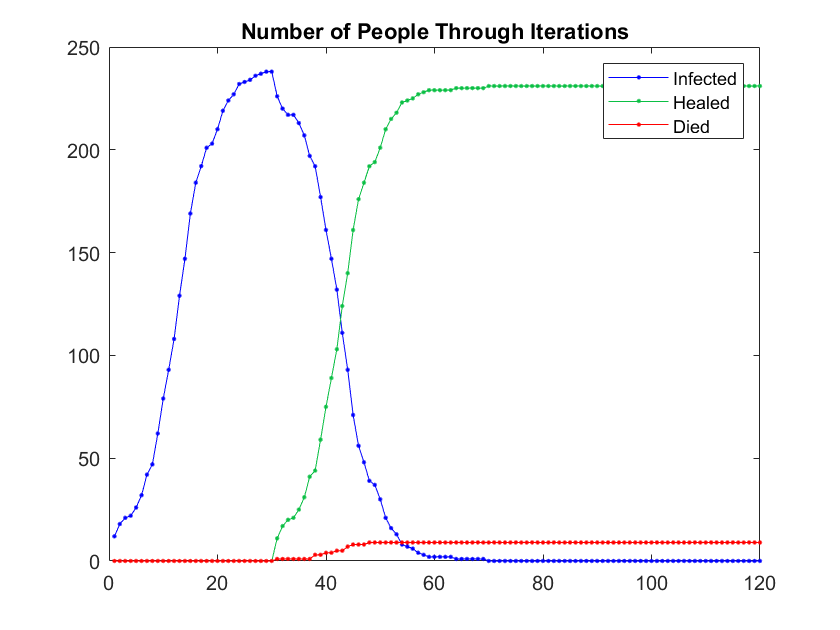
\includegraphics[width=5cm]{images/AlternativeScenarios/ScenarioI_IsolationProbability0.2_overall.png} }}%
    \qquad
    \subfloat[\centering Isolation Probability ($q_s$) = 0.5]{{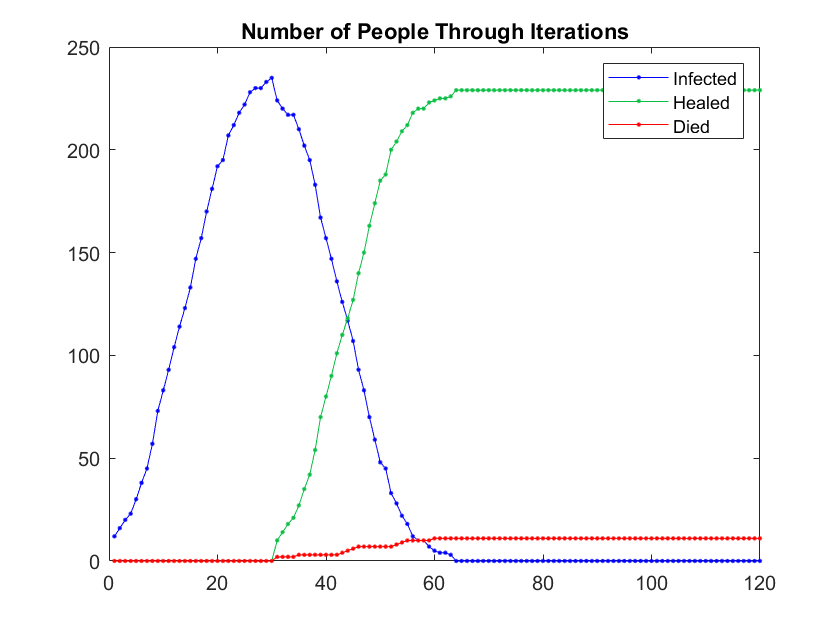
\includegraphics[width=5cm]{images/AlternativeScenarios/ScenarioI_IsolationProbability0.5_overall.png} }}%
    \qquad
    \subfloat[\centering Isolation Probability ($q_s$) = 0.8]{{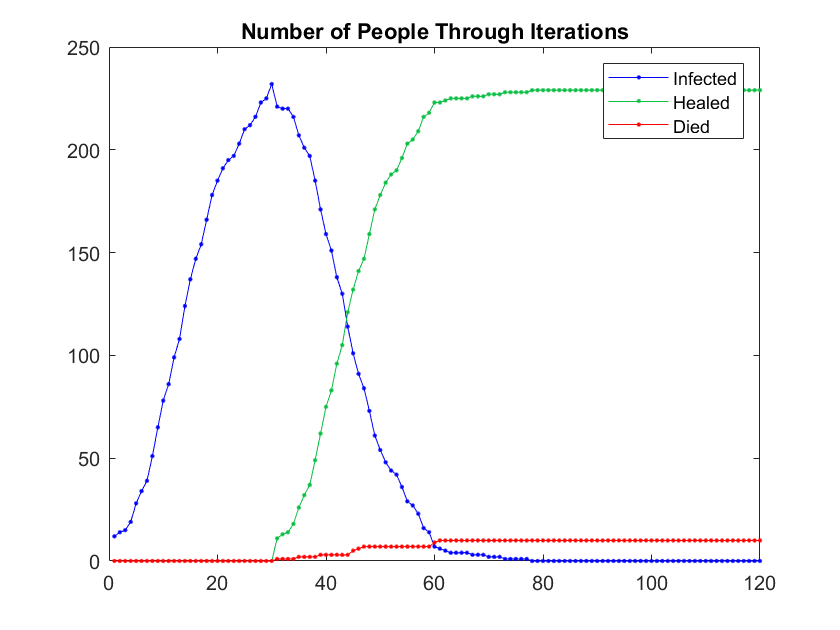
\includegraphics[width=5cm]{images/AlternativeScenarios/ScenarioI_IsolationProabability0.8_overall.png} }}%
    \caption{Total number of people in each iteration for different isolation probabilities}
    \label{fig:AlterQSSC1}%
\end{figure}

In all three cases, where the isolation probability is low, moderate, and high, all of the population gets infected. However, according to the number of people per iteration data (Figure \ref{fig:AlterQSSC1PerIter}), the number of iterations where the peak of infected people occurs and the peak value changes depending on the isolation probability. In Figure \ref{fig:AlterQSSC1PerIter}.a , where the isolation probability equals 20\%, the peak occurs earlier, closer to 15$^{\textrm{th}}$ iteration in the simulation. In contrast, in the case of the original scenario where the isolation probability equals 50\%, the peak of infected people occurs approximately at 20$^{\textrm{th}}$ iteration. In the case where isolation probability is equal to 80\%, the peak occurs approximately at the same iteration with the 50\% probability, but the span of the infected people per iteration is larger. Even after the 40$^{\textrm{th}}$ iteration, there are still new people getting infected. The reason behind this situation is due to the less iterations between infected and healthy people. The higher the isolation probability gets, the more people that have not been infected yet in the later iterations can still get infected. 

The peak values of the infected people in the case of isolation probability equal 20\% are higher than in other cases because more people get infected in a short amount of iterations. This situation might lead to some failure in the healthcare system.

The total number of dead people in all three cases is equal since, in all three situations, all of the population gets infected, and death probabilities are the same for people in the isolated and non-isolated infected people.

\begin{figure}[h]
    \centering
    \subfloat[\centering Isolation Probability ($q_s$) = 0.2]{{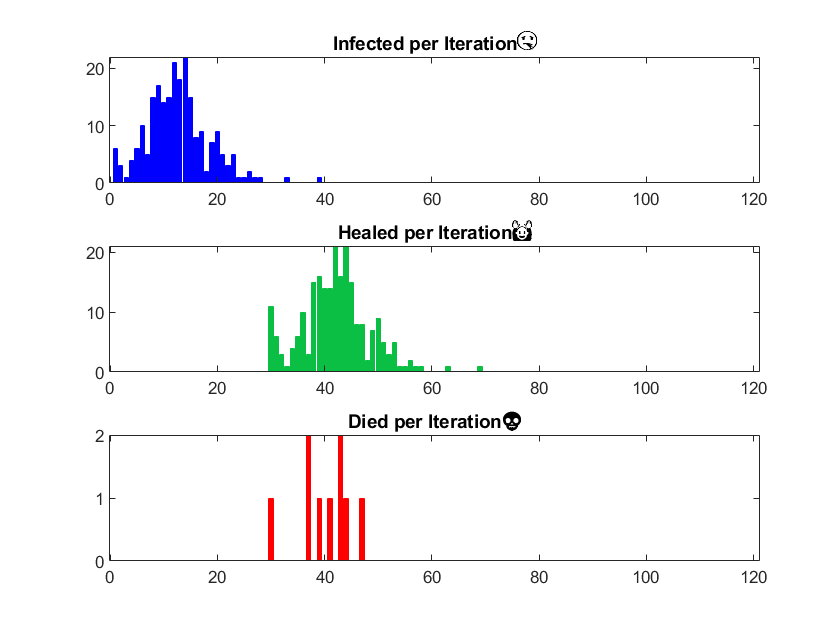
\includegraphics[width=5cm]{images/AlternativeScenarios/ScenarioI_IsolationProbability0.2_PerIteration.png} }}%
    \qquad
    \subfloat[\centering Isolation Probability ($q_s$) = 0.5]{{\includegraphics[width=5cm]{images/AlternativeScenarios/ScenarioI_IsolationProbsbility0.5_PerIteration.png} }}%
    \qquad
    \subfloat[\centering Isolation Probability ($q_s$) = 0.8]{{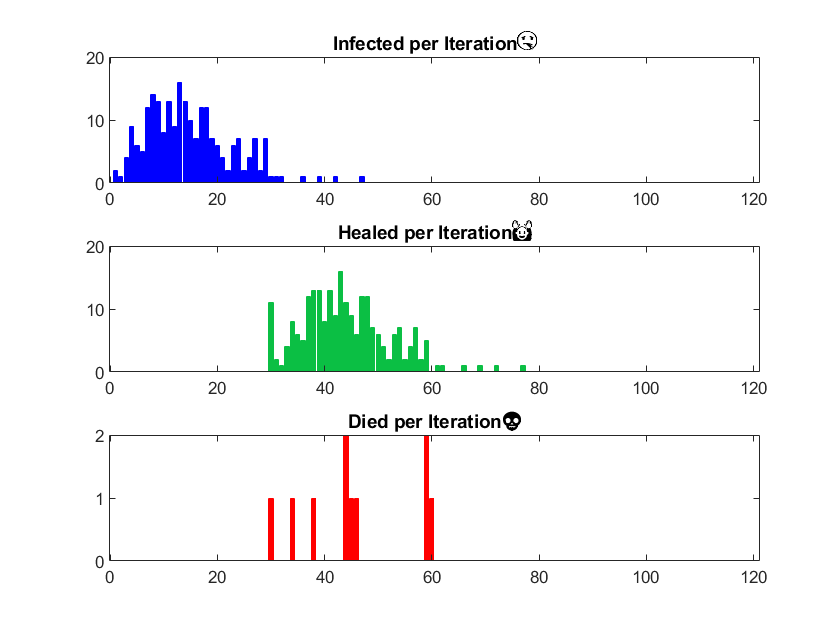
\includegraphics[width=5cm]{images/AlternativeScenarios/ScenarioI_IsolationProbability0.8_PerIteration.png} }}%
    \caption{Number of people in each iteration for different isolation probabilities}
    \label{fig:AlterQSSC1PerIter}%
\end{figure}

\newpage

\addcontentsline{toc}{subsection}{Vaccination Rate ( Scenario II )}
\subsection*{Vaccination Rate ( Scenario II )}

\; \; Under only the vaccination policy implemented, the effect of the vaccination rate is examined by changing the original vaccination rate function. 
$$
\\0.2\bigg(\frac{1}{t_v-19}\bigg)\leftarrow0.5\bigg(\frac{1}{t_v-19}\bigg)\rightarrow 0.8\bigg(\frac{1}{t_v-19}\bigg)\
$$

\begin{figure}[h]
    \centering
    \subfloat[\centering Vaccination Rate ($\Delta_3(t=20) = 0.2$)]{{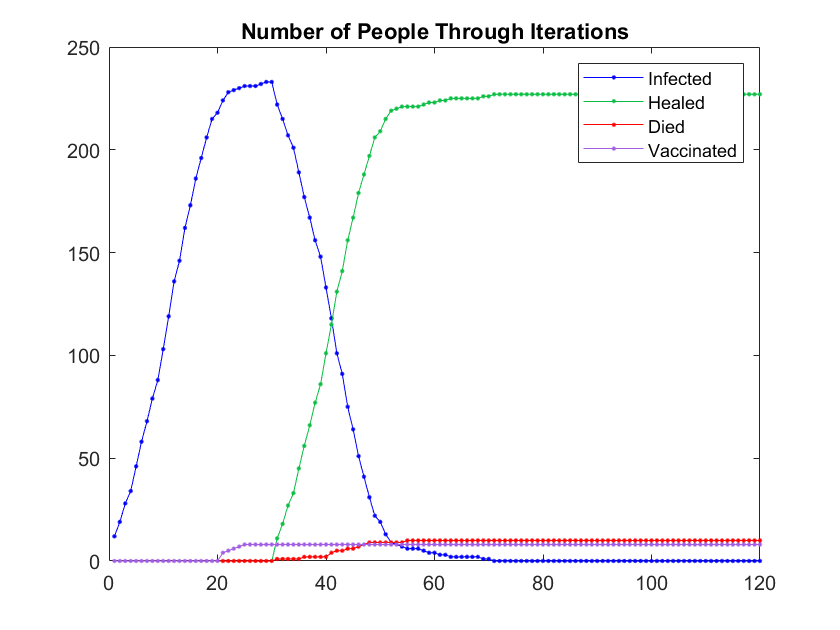
\includegraphics[width=6cm]{images/AlternativeScenarios/ScenarioII_VaccinationRate0.2_overall.png} }}%
    \qquad
    \subfloat[\centering Vaccination Rate ($\Delta_3(t=20) = 0.5$)]{{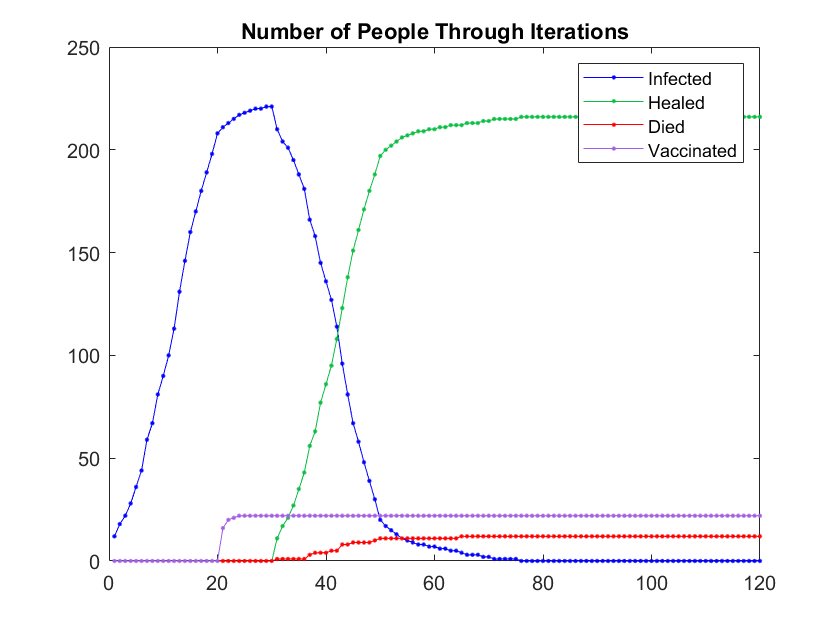
\includegraphics[width=6cm]{images/AlternativeScenarios/ScenarioII_VaccinationRate0.5_overall.png} }}%
    \qquad
    \subfloat[\centering Vaccination Rate ($\Delta_3(t=20) = 0.8$)]{{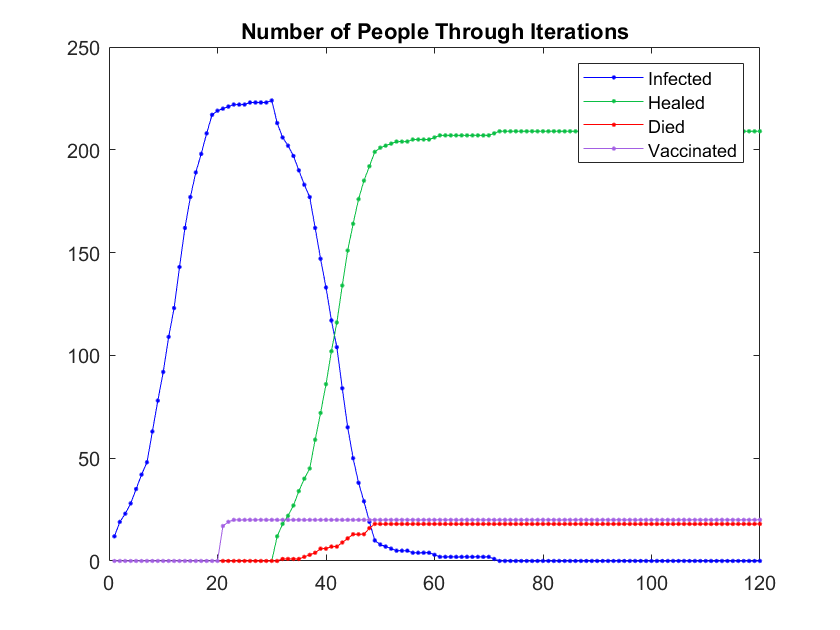
\includegraphics[width=6cm]{images/AlternativeScenarios/ScenarioII_VaccinationRate0.8_overall.png} }}%
    \caption{Total number of people in each iteration for different vaccination rate}
    \label{fig:AlterDelta3SC2all}%
\end{figure}
\begin{figure}
    \centering
    \subfloat[\centering Vaccination Rate ($\Delta_3(t=20) = 0.2$)]{{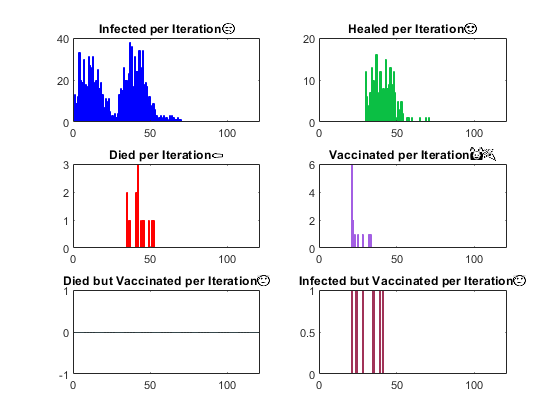
\includegraphics[width=6cm]{images/AlternativeScenarios/ScenarioII_VaccinationRate0.2_PerIteration.png} }}%
    \qquad
    \subfloat[\centering Vaccination Rate ($\Delta_3(t=20) = 0.5$)]{{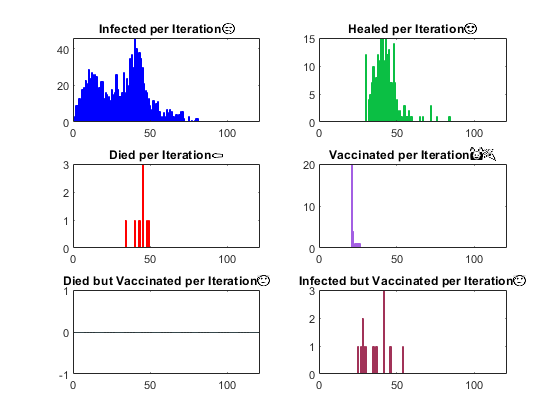
\includegraphics[width=6cm]{images/AlternativeScenarios/ScenarioII_VaccinationRate0.5_PerIteration.png} }}%
    \qquad
    \subfloat[\centering Vaccination Rate ($\Delta_3(t=20) = 0.8$)]{{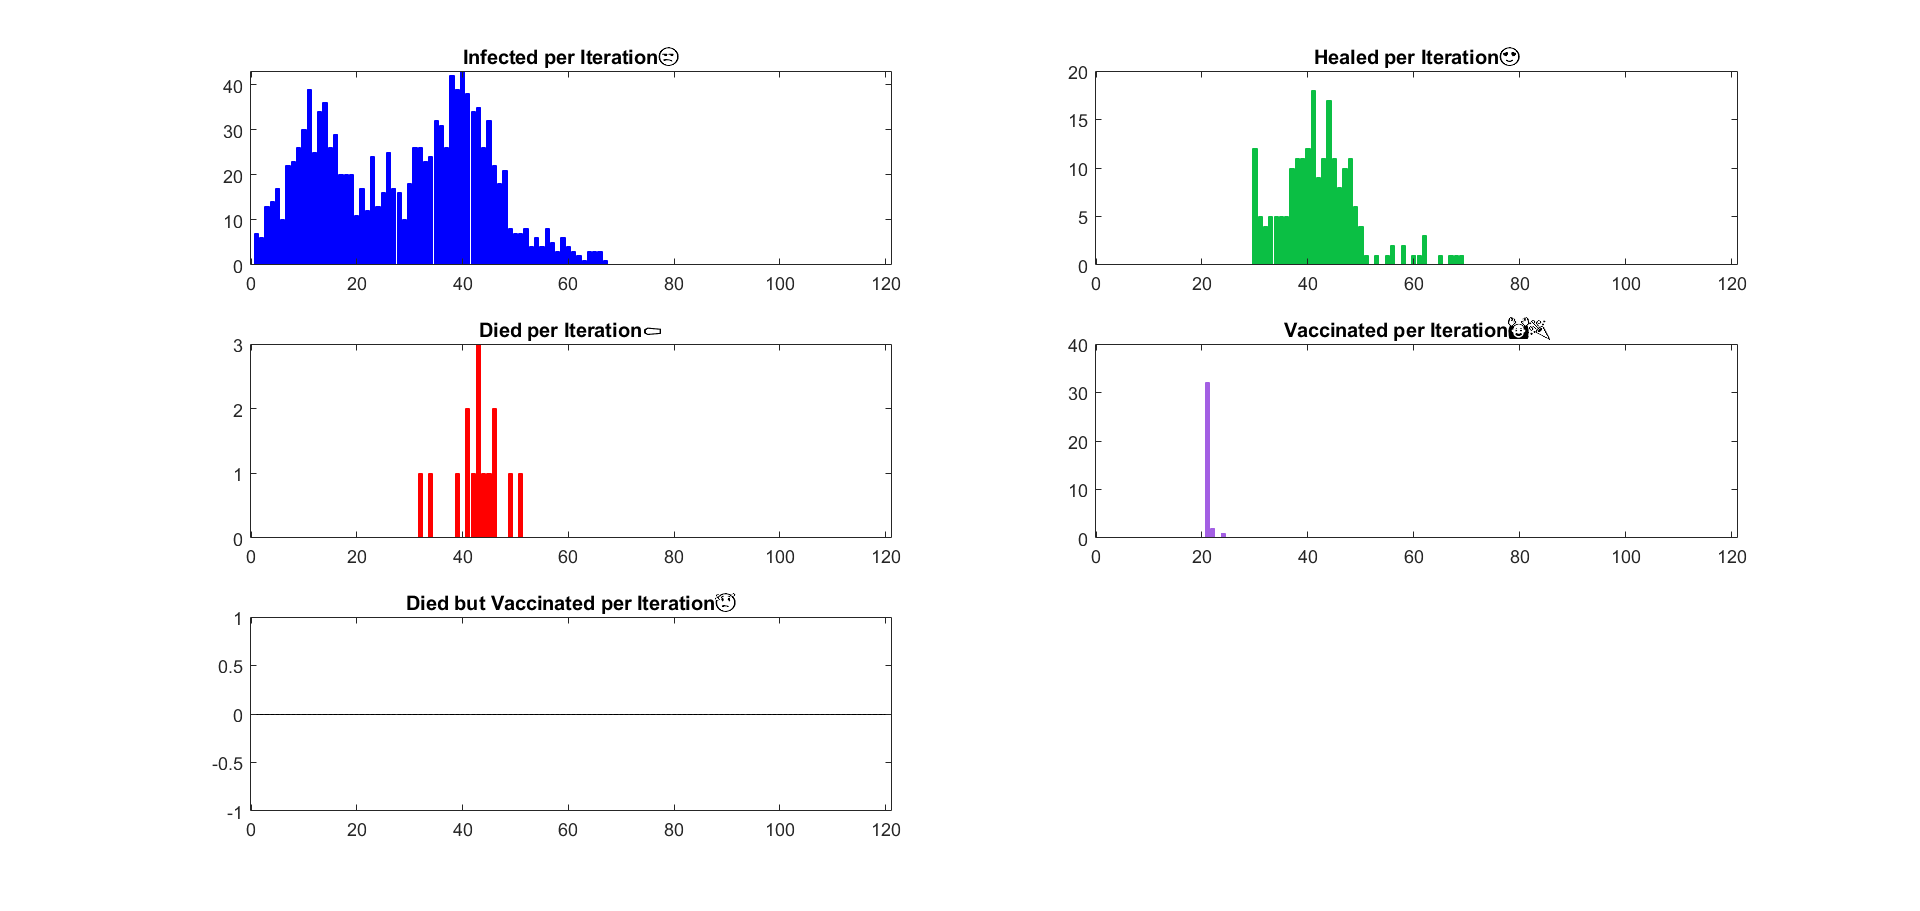
\includegraphics[width=6cm]{images/AlternativeScenarios/ScenarioII_VaccinationRate0.8_PerIteration.png} }}%
    \caption{Total number of people in each iteration for different vaccination rate}
    \label{fig:AlterDelta3SC2perIter}%
\end{figure}


According to the Figure \ref{fig:AlterDelta3SC2all}.a, where the vaccination rate of the population is lower, the more of the population gets infected, and even after the 20$^{\textrm{th}}$ iteration, the infection amount keeps growing, and eventually, all of the population gets infected. However, in the case of higher vaccination rates (Figure \ref{fig:AlterDelta3SC2all}.c) , after the 20$^{\textrm{th}}$ iteration,slope of the total infection curve decreases rapidly. This situation indicates that the spread of the virus can be controlled with higher rates of vaccination.

In all three cases where the vaccination rate is low, moderate, and high (Figure \ref{fig:AlterDelta3SC2perIter}), the pandemic unfolds in two waves. However, the peak of the waves is inversely proportional to the vaccination rate. In the case of a vaccination rate of 0.2, the peak of the second wave almost exceeds 50 people per iteration. In contrast, for the vaccination rates of 0.5 and 0.8, the peak occurs at around 40 people per iteration.

The total number of dead people is affected by the vaccination as well up to a certain threshold. For a rate of 0.5, the number of dead people is approximated as 11.47 in the 100 Monte-Carlo simulation. As the vaccination rate went down to 0.2, the number of dead people increased to 12.01. However, as the vaccination rate goes up to 0.8, the number of dead people is approximately equal to 11.5, which is almost the same as the vaccination rate of 0.5. This means that the speed of vaccination prevents deaths up to a certain level. 

\newpage

\addcontentsline{toc}{subsection}{Vaccination Rate ( Scenario III )}
\subsection*{Vaccination Rate ( Scenario III )}
\; \; Under the policy of vaccination and isolation together, keeping the isolation probability at its original value $q_s=0.5$, the effect of the vaccination rate is examined by changing the original vaccination rate function. 
$$
\\0.2\bigg(\frac{1}{t_v-19}\bigg)\leftarrow0.5\bigg(\frac{1}{t_v-19}\bigg)\rightarrow 0.8\bigg(\frac{1}{t_v-19}\bigg)\
$$

\begin{figure}[h]
    \centering
    \subfloat[\centering Vaccination Rate ($\Delta_3(t=20) = 0.2$)]{{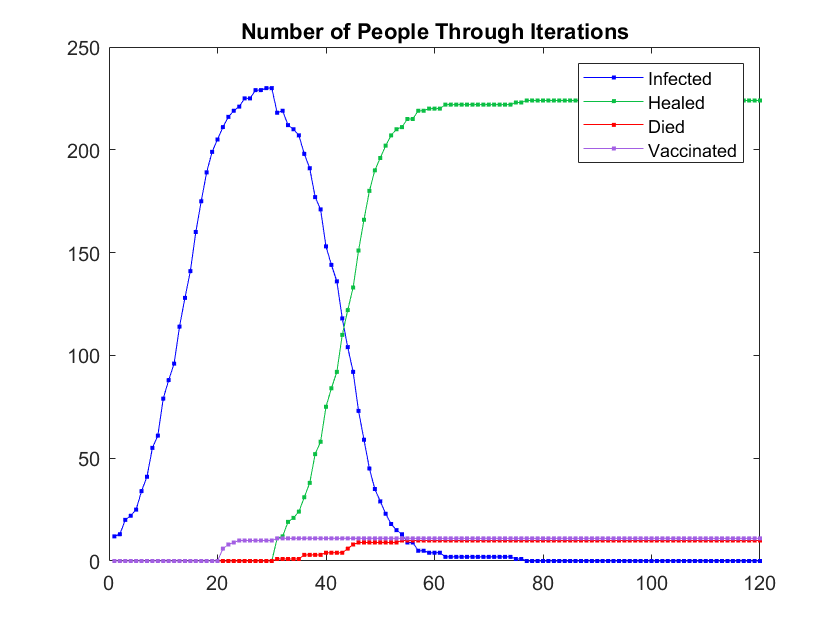
\includegraphics[width=6cm]{images/AlternativeScenarios/ScenarioIII_VaccinatedRate0.2_IsolationProbabilityConstant_overall.png} }}%
    \qquad
    \subfloat[\centering Vaccination Rate ($\Delta_3(t=20) = 0.5$)]{{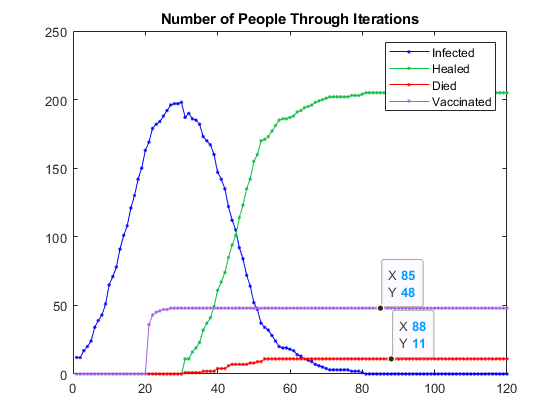
\includegraphics[width=6cm]{images/AlternativeScenarios/ScenarioIII_Isolation0.5Vaccination0.5_overall.png} }}%
    \qquad
    \subfloat[\centering Vaccination Rate ($\Delta_3(t=20) = 0.8$)]{{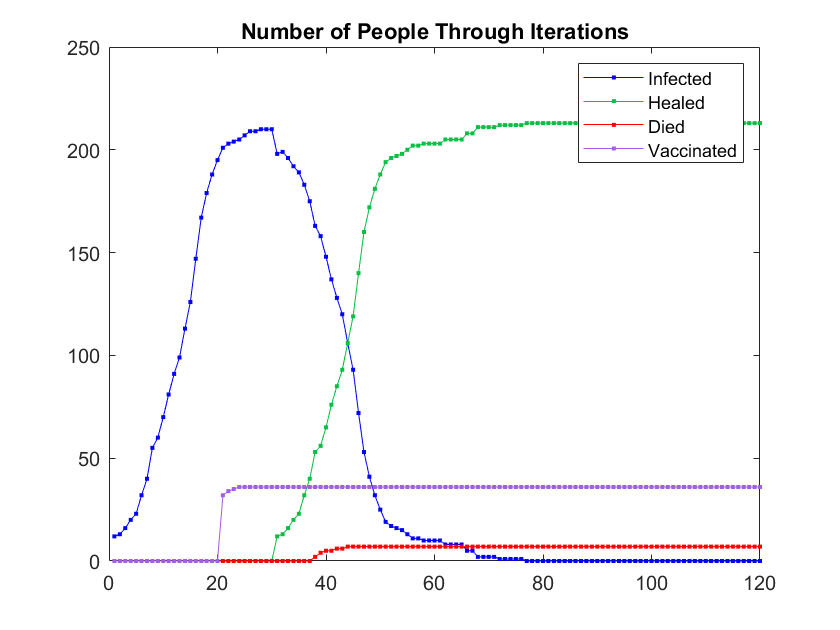
\includegraphics[width=6cm]{images/AlternativeScenarios/ScenarioIII_VaccinatedRate0.8_IsolationProbabilityConstant_overall.png} }}%
    \caption{Total number of people in each iteration for different isolation rate}
    \label{fig:AlterDelta3SC3all}%
\end{figure}

As can be seen in Figure \ref{fig:AlterDelta3SC3all}.a, when the vaccination rate is 20\%, almost all of the population gets infected around the same time. And this brings the pandemic to a fast conclusion. This many cases around the same time might lead to failure in the healthcare system. In contrast, when the vaccination rate increases to 80\% (Figure \ref{fig:AlterDelta3SC3all}.c), some people in the population is not even infected. Also, the pandemic unfolds over a longer time period. In Figure \ref{fig:AlterDelta3SC3all}.a, it can be seen that starting from the 60$^{\textrm{th}}$ iteration,there is no new cases of infection. But in Figure \ref{fig:AlterDelta3SC3all}.b and Figure \ref{fig:AlterDelta3SC3all}.c, this number reaches to almost 80$^{\textrm{th}}$ iteration. Similar to Alternative for Scenario II, where the vaccination rate is high, the slope of the infection curve decreases compared to the same scenario with a lower vaccination rate.

According to Figure \ref{fig:AlterDelta3SC3all}, as the vaccination rate becomes higher, the number of dead people decreases. This situation can be seen clearly by comparing each graph in Figure \ref{fig:AlterDelta3SC3all}. In the case where isolation probability is kept as constant and vaccination rate is decreased to 20\%, (Figure \ref{fig:AlterDelta3SC3all}.a), people died in total on average is more than vaccination rate of 0.8 with the same isolation probability (Figure \ref{fig:AlterDelta3SC3all}.c) . In the case of vaccination probability 20\%, number of dead people is equal to 17 (Figure \ref{fig:AlterDelta3SC3all}.a) whereas when vaccination probability increases to 50\%, that value decreases to 11(Figure \ref{fig:AlterDelta3SC3all}.b). Even though this correlation applies until a certain threshold, if the vaccination rate keeps increasing under the same isolation probability, the total number of dead people is not affected significantly, similar to the Alternative Scenario II (Figure \ref{fig:AlterDelta3SC3all}.c).

\newpage

\addcontentsline{toc}{subsection}{Isolation Rate ( Scenario III )}
\subsection*{Isolation Rate ( Scenario III )}

\; \; Under the policy of vaccination and isolation together, keeping the vaccination rate at its original value according to the function $\frac{1}{2*(t_v-19)}$ , the effect of infection probability is examined by changing the original probability $q_s=0.5$.

\begin{figure}[h]
    \centering
    \subfloat[\centering Isolation Probability ($q_s = 0.2$)]{{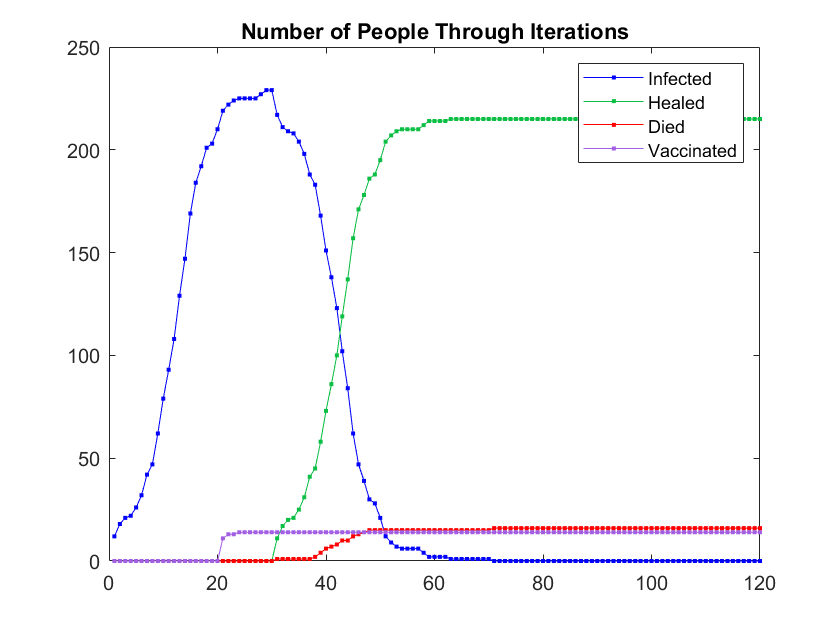
\includegraphics[width=5cm]{images/AlternativeScenarios/ScenarioIII_IsolationProbability0.2_VaccinatedRateConstant_overall.png} }}%
    \qquad
    \subfloat[\centering Isolation Probability ($q_s = 0.5$)]{{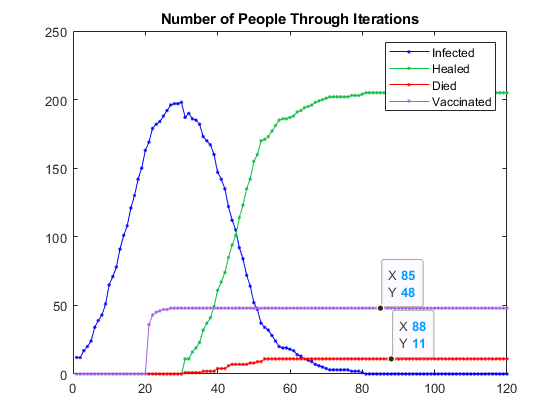
\includegraphics[width=5cm]{images/AlternativeScenarios/ScenarioIII_Isolation0.5Vaccination0.5_overall.png} }}%
    \qquad
    \subfloat[\centering Isolation Probability ($q_s = 0.8$)]{{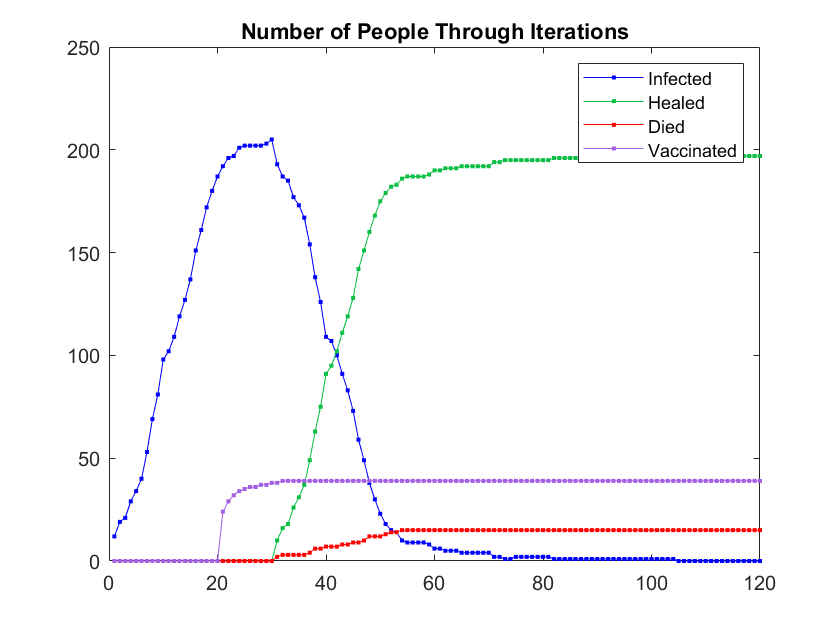
\includegraphics[width=5cm]{images/AlternativeScenarios/ScenarioIII_IsolationProbability0.8_VaccinatedRateConstant_overall.png} }}%
    \caption{Total number of people in each iteration for different isolation probability}
    \label{fig:AlterQsSC3all}%
\end{figure}

The lower isolation probability under the same vaccination rate affects both the total number of infections and the total number of vaccination. As the number of interactions between people increases due to the low isolation probability, the total number of infections increases in earlier iterations. Because of this, there will be fewer healthy people to vaccinate when the vaccination starts. This can be seen by comparing the vaccination amounts in (Figure \ref{fig:AlterQsSC3all}.a) and (Figure \ref{fig:AlterQsSC3all}.c). The total number of infected people in the case where isolation probability equals 80\% is lower than 200. This number increases to 240 when the probability equals 20\%.

The total number of dead people is also affected by the changing isolation probabilities under the same vaccination rates. As the isolation probability increases, the total number of dead people decreases since there will be less interaction and less chance of getting infected in the first place.

\addcontentsline{toc}{subsection}{Second Vaccination Rate ( Scenario IV )}
\subsection*{Second Vaccination Rate ( Scenario IV )}
\; \; Under the double vaccination scenario, given the isolation probability in Scenario I ($q_S=0.5$), the effect of the second vaccination rate is examined by changing the original rate $w=0.8$.

\begin{figure}[h]
    \centering
    \subfloat[\centering Vaccination Rate ($w = 0.2$)]{{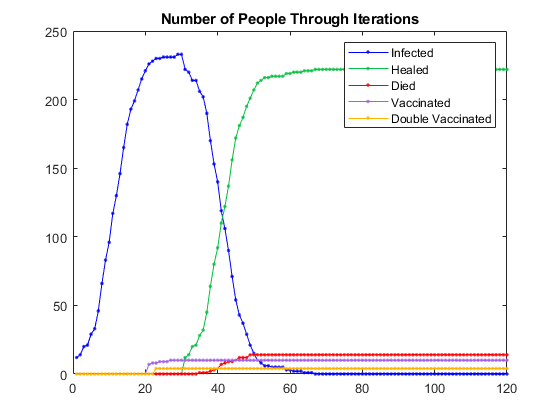
\includegraphics[width=6cm]{images/AlternativeScenarios/ScenarioIV_SecondVaccinationProbability0.2_overall.png} }}%
    \qquad
    \subfloat[\centering Vaccination Rate ($w = 0.5$)]{{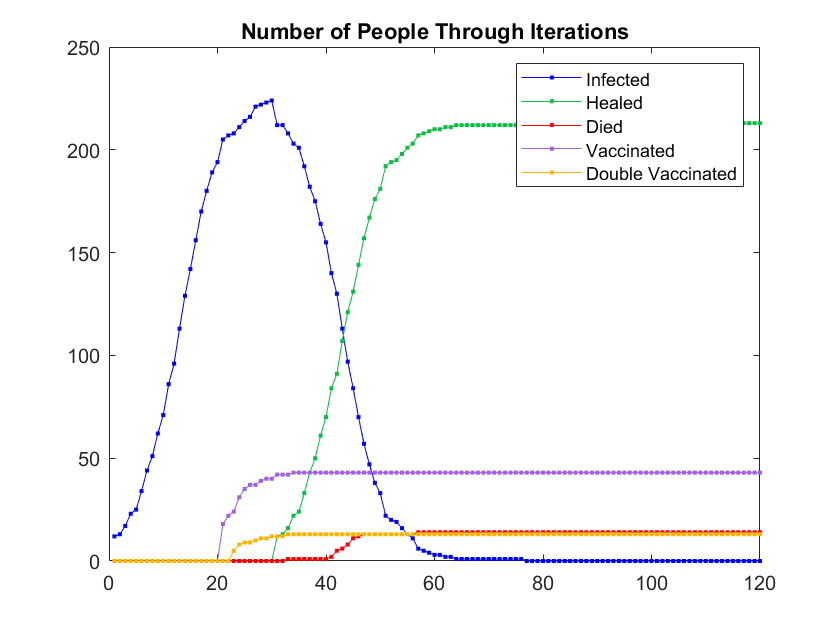
\includegraphics[width=6cm]{images/AlternativeScenarios/ScenarioIV_SecondVaccinationProbability0.5_overall.png} }}%
    \qquad
    \subfloat[\centering Vaccination Rate ($w = 0.8$)]{{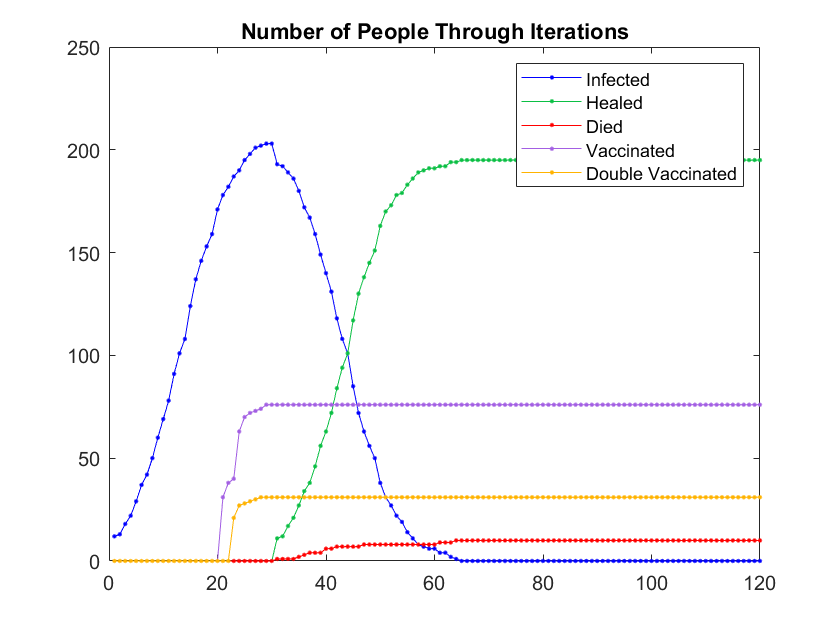
\includegraphics[width=6cm]{images/AlternativeScenarios/ScenarioIV_SecondVaccinationRate0.8_overall.png} }}%
    \caption{Total number of people in each iteration for different second dose vaccination rate}
    \label{fig:AlterSC4}%
\end{figure}

By looking at Figure \ref{fig:AlterSC4}, infection rates seem dependent on the second dose vaccination rate. However, since vaccination and double vaccination start after 20$^{\textrm{th}}$ iteration, until iteration 20, the total number of infected people is solely dependent on the random movement of individuals. After the 20$^{\textrm{th}}$ iteration, as the vaccination and second vaccination starts, in the case of lower second vaccination rates (Figure \ref{fig:AlterSC4}.a), more of the population gets infected comparing to the higher second vaccination rates (Figure \ref{fig:AlterSC4}.c).

The total number of dead people is also affected by the change in the second vaccination rates under the same isolation probability as in Scenario I. According to (Figure \ref{fig:AlterSC4}.a), the number of total dead people is higher when the second vaccination rate is decreased to 20\%, compared to the case where the second vaccination rate is 80\%.(Figure \ref{fig:AlterSC4}.c). This correlation can also be guaranteed by checking the second vaccination rate of 50\% under the same isolation probability(Figure \ref{fig:AlterSC4}.b). The total number of dead people takes place in the middle of lower and higher second vaccination rates(20\% and 80\% respectively). This means that higher rates of second vaccination prevent deaths if an isolation policy is implemented at the same time.
\newpage
\addcontentsline{toc}{section}{Conclusion}
\section*{Conclusion}
\;\;\;\;\;\;In this project, we simulated the spread of the Coronavirus and its effects on the population under different restrictions and policies. Decision-makers could implement different policies based on findings from the simulation.

One of the findings of this simulation is that, for earlier stages of the pandemic, isolation holds a great role in reducing the spread of the virus. With higher isolation rates, the virus could be controlled with ease until the vaccination starts. In Scenarios I and III, the impact of isolation can be seen in the total number of infections. Strict isolation policies would be a wise decision in the earlier stages of the pandemic. In the alternative scenario for Scenario III, where the isolation rate is higher, a fall in the total number of infected people can easily be seen.

Since the spread of the virus is reduced by isolation, more people will be eligible for the vaccination. In the scenarios where both isolation and vaccination are implemented, after the 20$^{\textrm{th}}$ iteration total number of people who got vaccinated is greater than in scenarios with no isolation policy is implemented. Since more people are vaccinated in the late stages of the pandemic, total death rates will be slim, and the possibility of a second wave will be way less. 

For further protection against late-stage deaths and infections, double vaccination would be a great deal-breaker. Since many of the late pandemic death and infection are caused by partial protection of first dose vaccination, doubling it and making each individual totally protected against the virus will stop most of the deaths after the vaccination starts.

In conclusion, if a government wants to take the pandemic under control and reduce the total deaths to a minimum, it should apply strict isolation policies to prevent new infections and encourage each and every one of the citizens to take both doses of vaccination to reduce the number of deaths.

\newpage
\thispagestyle{empty}

\section*{Appendix}

\begin{figure}[h]
    \centering
    \subfloat[\centering Vaccination Rate ($\Delta_3(t=20) = 0.2$)]{{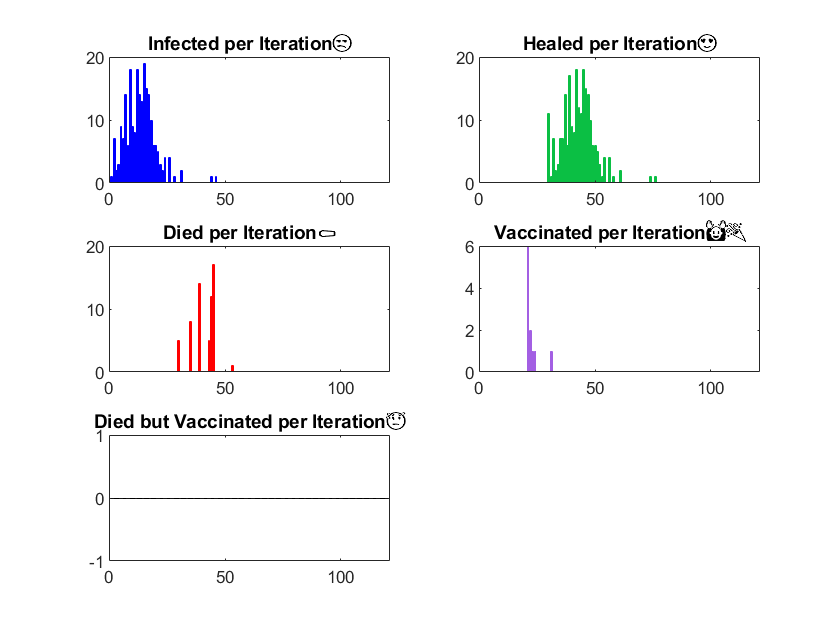
\includegraphics[width=5cm]{images/AlternativeScenarios/ScenarioIII_VaccinatedRate0.2_IsolationProbabilityConstant_PerIteration.png} }}%
    \qquad
    \subfloat[\centering Vaccination Rate ($\Delta_3(t=20) = 0.5$)]{{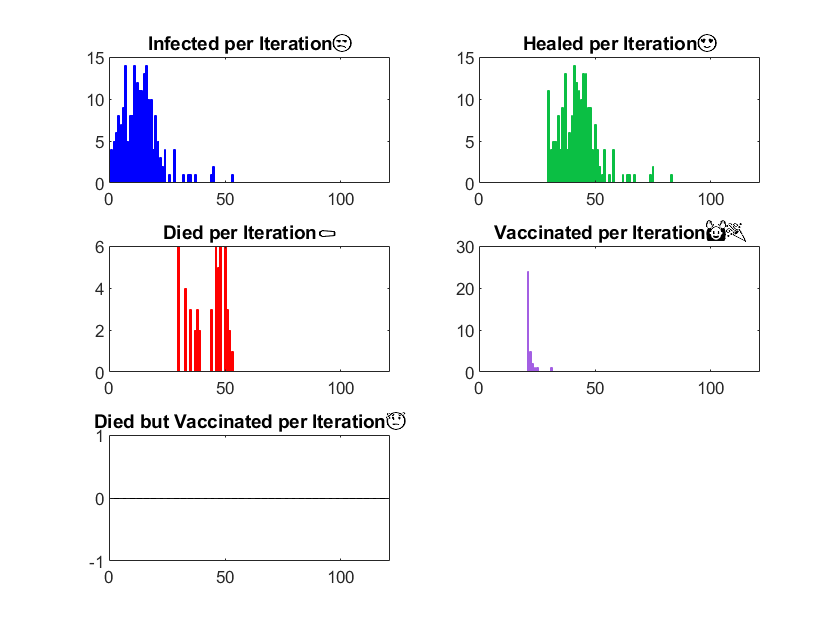
\includegraphics[width=5cm]{images/AlternativeScenarios/ScenarioIII_Isolation0.5Vaccination0.5PerIteration.png} }}%
    \qquad
    \subfloat[\centering Vaccination Rate ($\Delta_3(t=20) = 0.8$)]{{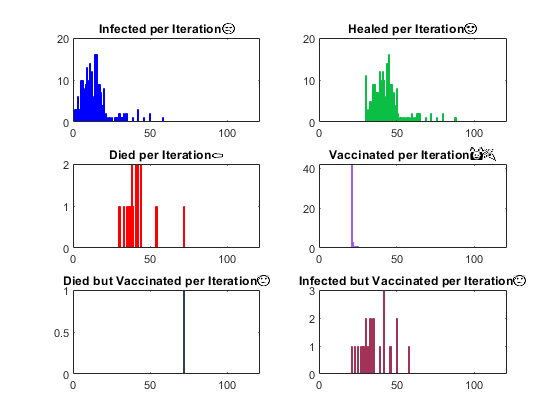
\includegraphics[width=5cm]{images/AlternativeScenarios/ScenarioIII_VaccinatedRate0.8_IsolationProbabilityConstant_PerIteration.png} }}%
    \caption{Number of people per iteration for different vaccination rate (Alternative for Scenario III)}
\end{figure}


\begin{figure}[h]
    \centering
    \subfloat[\centering Isolation Probability ($q_s = 0.2$)]{{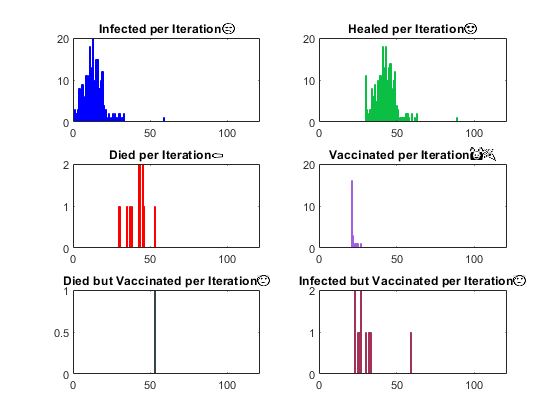
\includegraphics[width=5cm]{images/AlternativeScenarios/ScenarioIII_IsolationProbability0.2_VaccinatedRateConstant_PerIteration.png} }}%
    \qquad
    \subfloat[\centering Isolation Probability ($q_s = 0.5$)]{{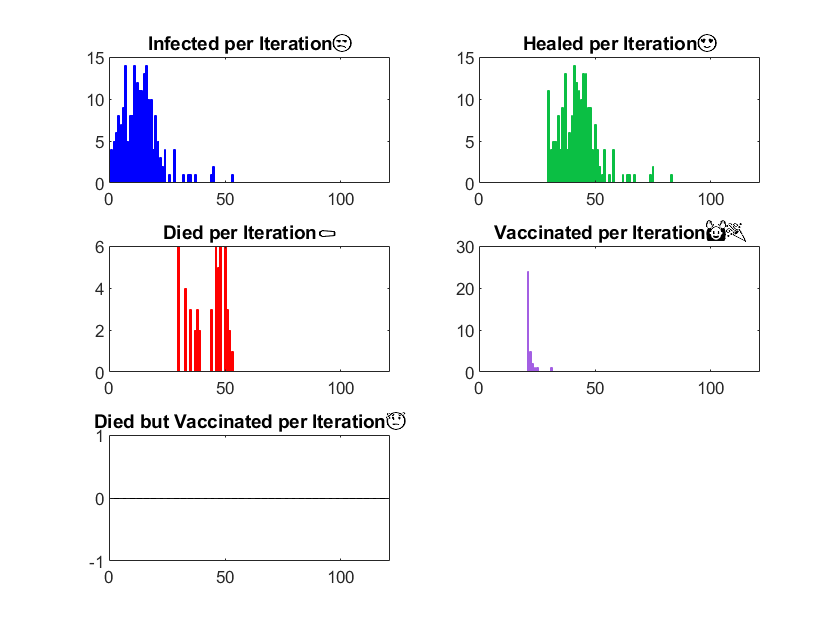
\includegraphics[width=5cm]{images/AlternativeScenarios/ScenarioIII_Isolation0.5Vaccination0.5PerIteration.png} }}%5
    \qquad
    \subfloat[\centering Isolation Probability ($q_s = 0.8$)]{{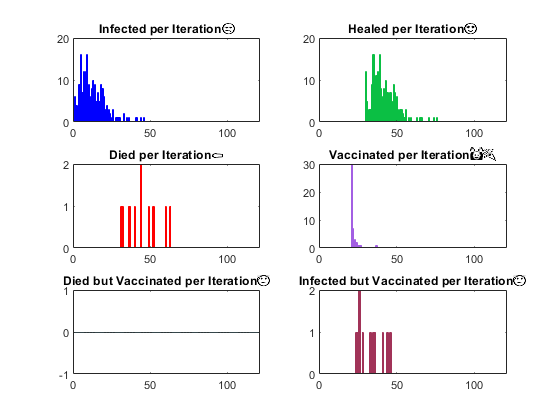
\includegraphics[width=5cm]{images/AlternativeScenarios/ScenarioIII_IsolationProbability0.8_VaccinatedRateConstant_PerIteration.png} }}%
    \caption{Number of people per iteration for different isolation probability (Alternative for Scenario III)}
\end{figure}


\begin{figure}[h]
    \centering
    \subfloat[\centering Vaccination Rate ($w = 0.2$)]{{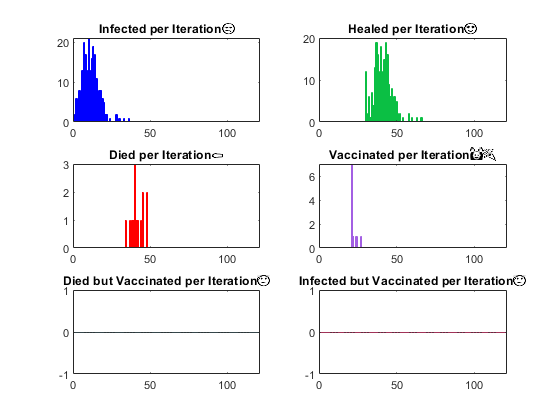
\includegraphics[width=5cm]{images/AlternativeScenarios/ScenarioIV_SecondVaccinationProbability0.2_PerIteration.png} }}%
    \qquad
    \subfloat[\centering Vaccination Rate ($w = 0.5$)]{{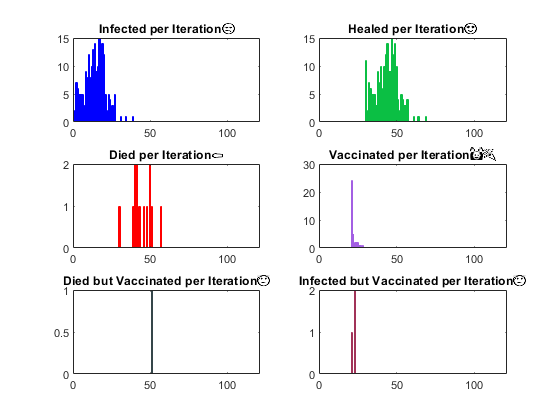
\includegraphics[width=5cm]{images/AlternativeScenarios/ScenarioIV_SecondVaccinationProbability0.5_PerIteration.png} }}%
    \qquad
    \subfloat[\centering Vaccination Rate ($w = 0.8$)]{{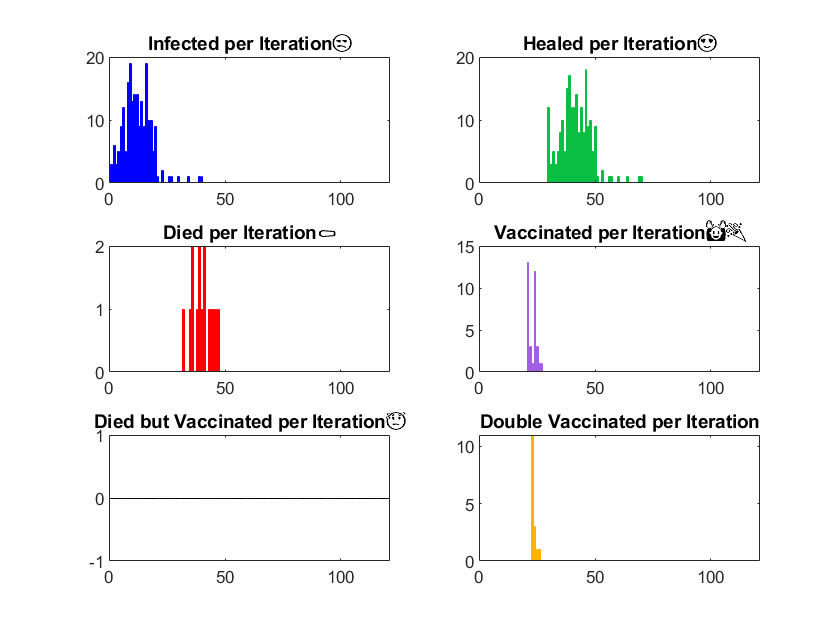
\includegraphics[width=5cm]{images/AlternativeScenarios/ScenarioIV_SecondVaccinationRate0.8_PerIteration.png} }}%
    \caption{Number of people per iteration for different second dose vaccination rate (Alternative for Scenario IV)}
\end{figure}
\begin{figure}[h!]
    \centering
    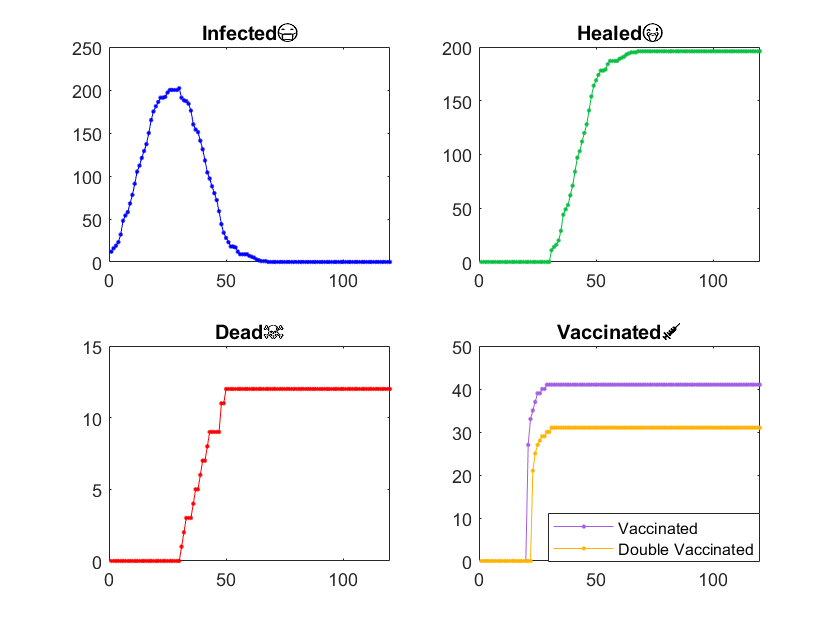
\includegraphics[width=5cm]{images/ScenarioIV_split.png}
    \caption{Total number of people in Scenario IV shown in separate graphs }
\end{figure}



\end{document}
